\newpage
\section{Protocole - Remplacer l'eau des chillers}
\label{a:chillers}

\textbf{N.B. Prévoir un seau pour vider les conduits et le chiller pour ne pas inonder le laboratoire. Traitement à effectuer tous les 3 mois.}

\subsection*{Remplacer l'eau des conduits}
Remplacer l'eau du chiller ne suffit pas à retirer toute l'eau du système. De l'eau s'est également accumulée dans les conduits des cavités laser et il faut les vider.
\begin{enumerate}
\item Éteindre le laser si ce n'est pas déjà fait
\item Éteindre le chiller
\item Retirer les tuyaux et les déposer dans un contenant pour recueillir l'eau des conduits
\item Vider le chiller de son eau
\item Mettre 400 ml d'eau doublement distillée (très important de mettre l'eau désionisée et déminéralisée)
\item Reconnecter le tout et rallumer le chiller
\item Laisser tourner l'eau pendant une dizaine de minutes
\item Répéter 1-2 fois
\end{enumerate}

\subsection*{Produit anticorrosif}
Le produit anticorrosif provient de la compagnie "OptiTemp". Le produit est OptiShield Plus. C'est un produit spécifiquement fait pour protéger les circuits d'eau fermés de la corrosion. Il protège des contaminants que contiennent l'aluminium, le bronze, le cuivre et tout type de métaux si ceux-ci sont présents dans le circuit. Une photo mise à la fin du document donne une description du produit.
\begin{enumerate}
\item Prendre environ 40 ml du produit anticorrosif
\item Ajouter 400 ml d'eau désionisée et déminéralisée (doublement distillé)
\item Remplir le chiller avec la solution
\item Allumer le chiller et laisser remplir les tuyaux de la solution
\item Ajouter le reste de la solution s'il en reste (le niveau d'eau a diminué pour remplir les conduits de la cavité laser)
\end{enumerate}

\begin{figure}[t!]
\centering
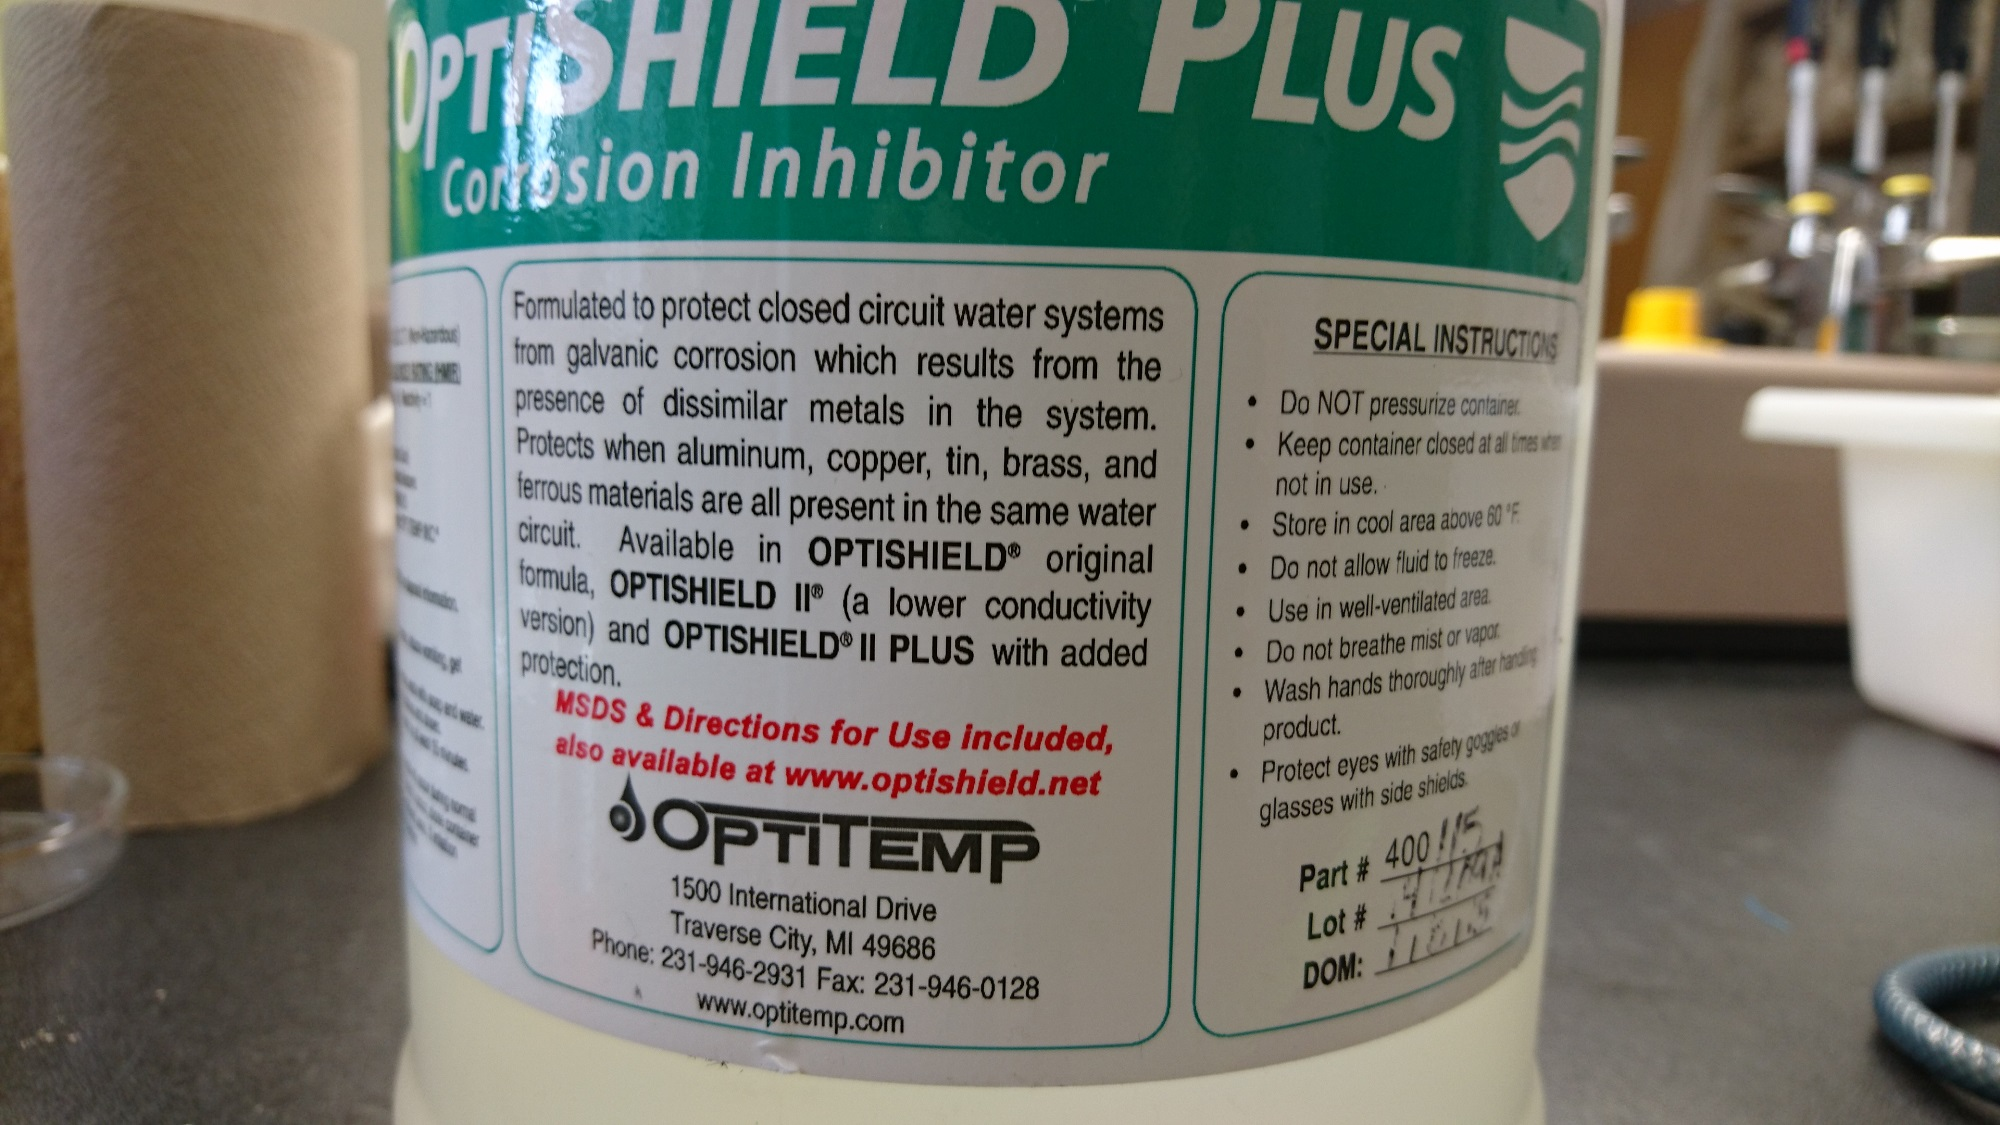
\includegraphics[scale=0.2]{anticorrosif_chiller.jpg}
\end{figure}